\documentclass[aspectratio=169, table]{beamer}

%\usepackage[beamertheme=./praditatheme]{Pradita}
\usepackage[utf8]{inputenc}
\usepackage{xcolor} % for color
\usepackage{colortbl} % for table color
\usepackage{listings}

% Define Java language style for listings
\lstdefinestyle{JavaStyle}{
language=Java,
basicstyle=\ttfamily\scriptsize,
keywordstyle=\color{blue},
commentstyle=\color{gray},
stringstyle=\color{red},
breaklines=true,
showstringspaces=false,
tabsize=2,
captionpos=b,
numbers=left,
numberstyle=\tiny\color{gray},
frame=lines,
backgroundcolor=\color{lightgray!10},
comment=[l]{//},
morecomment=[s]{/*}{*/},
commentstyle=\color{gray}\ttfamily,
string=[s]{'}{'},
morestring=[s]{"}{"},
%	stringstyle=\color{teal}\ttfamily,
%	showstringspaces=false
}

\usetheme{Pradita}
%
\subtitle{IF220303 - Object-oriented Programming}

\title{\Huge{Structural Patterns 2}\\\vspace{30pt}}
\date[Serial]{\scriptsize {PRU/SPMI/FR-BM-18/0222}}
\author[Pradita]{\small {\textbf{Alfa Yohannis}}}

\begin{document}

\frame{\titlepage}

\begin{frame}[fragile]
\frametitle{Contents}
\vspace{20pt}
\begin{columns}[t]
\column{0.5\textwidth}
\tableofcontents[sections={1-2}]

\column{0.5\textwidth}
\tableofcontents[sections={3-4}]
\end{columns}
\end{frame}


\section{Pola Struktural (Bagian 2)}

\begin{frame}{Pola Struktural Lanjutan}
	\vspace{10pt}
	Pola struktural lanjutan meliputi pola yang membantu menyederhanakan struktur antar objek dan memfasilitasi komunikasi yang efisien dalam sistem yang kompleks. 
	
	\vspace{10pt}
	Bab ini mencakup tiga pola desain penting:
	\begin{itemize}
		\item \textbf{Facade:} Menyediakan antarmuka tunggal untuk menyederhanakan akses ke subsistem kompleks.
		\item \textbf{Proxy:} Mengontrol akses ke objek dengan menyediakan perantara yang mewakili objek asli.
		\item \textbf{Flyweight:} Menghemat memori dengan berbagi instansi objek yang identik dan tidak berubah.
	\end{itemize}
	
	\vspace{5pt}
	Implementasi yang tepat dari pola-pola ini mendukung efisiensi arsitektur, modularitas sistem, dan pengelolaan kompleksitas kode.
\end{frame}


\section{Pola Facade}

\begin{frame}{\hfill}
	\centering
	\textbf{\Huge{Pola Facade}}
\end{frame}

\begin{frame}{Facade: Tujuan dan Konteks Penggunaan}
	\vspace{20pt}
	\begin{columns}[T]
		\column{0.5\textwidth}
		\textbf{Deskripsi:} \\
		Pola \textit{Facade} menyederhanakan interaksi dengan subsistem kompleks melalui antarmuka tunggal. Cocok untuk sistem besar dengan banyak modul dan dependensi.
		
		\vspace{8pt}
		\textbf{Tujuan:}
		\begin{itemize}
			\item Menyederhanakan akses ke subsistem.
			\item Mengurangi ketergantungan langsung.
			\item Memisahkan tanggung jawab antar modul.
		\end{itemize}
		
		\column{0.5\textwidth}
		\textbf{Kapan Digunakan:}
		\begin{itemize}
			\item Klien hanya perlu sebagian fungsi.
			\item Perlu integrasi antarmuka sederhana.
			\item Ingin meningkatkan maintainability dan isolasi.
		\end{itemize}
		
		\vspace{6pt}
		\textbf{Analogi:} \\
		Seperti resepsionis hotel—satu titik akses ke banyak layanan tanpa tahu struktur internal hotel.
	\end{columns}
\end{frame}



\begin{frame}{Facade: Contoh Kasus Penggunaan}
	\vspace{20pt}
	\begin{columns}[T]
		\column{0.5\textwidth}
		\textbf{Contoh 1: Pemesanan Tiket Online}
		\begin{itemize}
			\item \texttt{UserAccountService}, \texttt{PaymentService}, \texttt{SeatReservationService}, \texttt{NotificationService}.
			\item \texttt{BookingFacade.bookTicket()} menyederhanakan semua pemanggilan.
		\end{itemize}
		
		\vspace{6pt}
		\textbf{Contoh 2: Kompilasi dalam IDE}
		\begin{itemize}
			\item Parsing, analisis, optimisasi, kompilasi.
			\item Tombol “Compile” = facade untuk seluruh proses.
		\end{itemize}
		
		\column{0.5\textwidth}
		\textbf{Contoh 3: Laporan Keuangan ERP}
		\begin{itemize}
			\item Data dari modul inventori, transaksi, akuntansi.
			\item \texttt{ReportFacade} menyatukan proses pelaporan.
		\end{itemize}
		
		\vspace{6pt}
		\textbf{Contoh Lain:}
		\begin{itemize}
			\item \texttt{ComputerFacade}
			\item \texttt{HomeTheaterFacade}
			\item \texttt{StartupFacade}
		\end{itemize}
	\end{columns}
\end{frame}

\begin{frame}{Facade: Kelebihan dan Kekurangan}
	\vspace{20pt}
	\begin{columns}[t]
		\column{0.5\textwidth}
		\textbf{Kelebihan:}
		\begin{itemize}
			\item Menyederhanakan antarmuka sistem dengan titik masuk tunggal.
			\item Meningkatkan \textit{decoupling} antara klien dan subsistem.
			\item Memfasilitasi standarisasi urutan dan validasi proses.
			\item Mempermudah penggunaan sistem besar yang kompleks.
			\item Cocok untuk integrasi antar-layer (MVC, mikrosistem).
		\end{itemize}
		
		\column{0.5\textwidth}
		\textbf{Kekurangan:}
		\begin{itemize}
			\item Abstraksi bisa terlalu sempit dan menyembunyikan fitur penting.
			\item Risiko duplikasi logika dari subsistem ke facade.
			\item Menambah overhead arsitektur dalam kasus kecil.
			\item Klien terlalu bergantung pada facade, menyulitkan pengujian.
			\item Tidak menyederhanakan subsistem internal—hanya menyembunyikan.
		\end{itemize}
	\end{columns}
\end{frame}


\begin{frame}{Struktur Pola Facade}
	\vspace{20pt}
	\begin{center}
		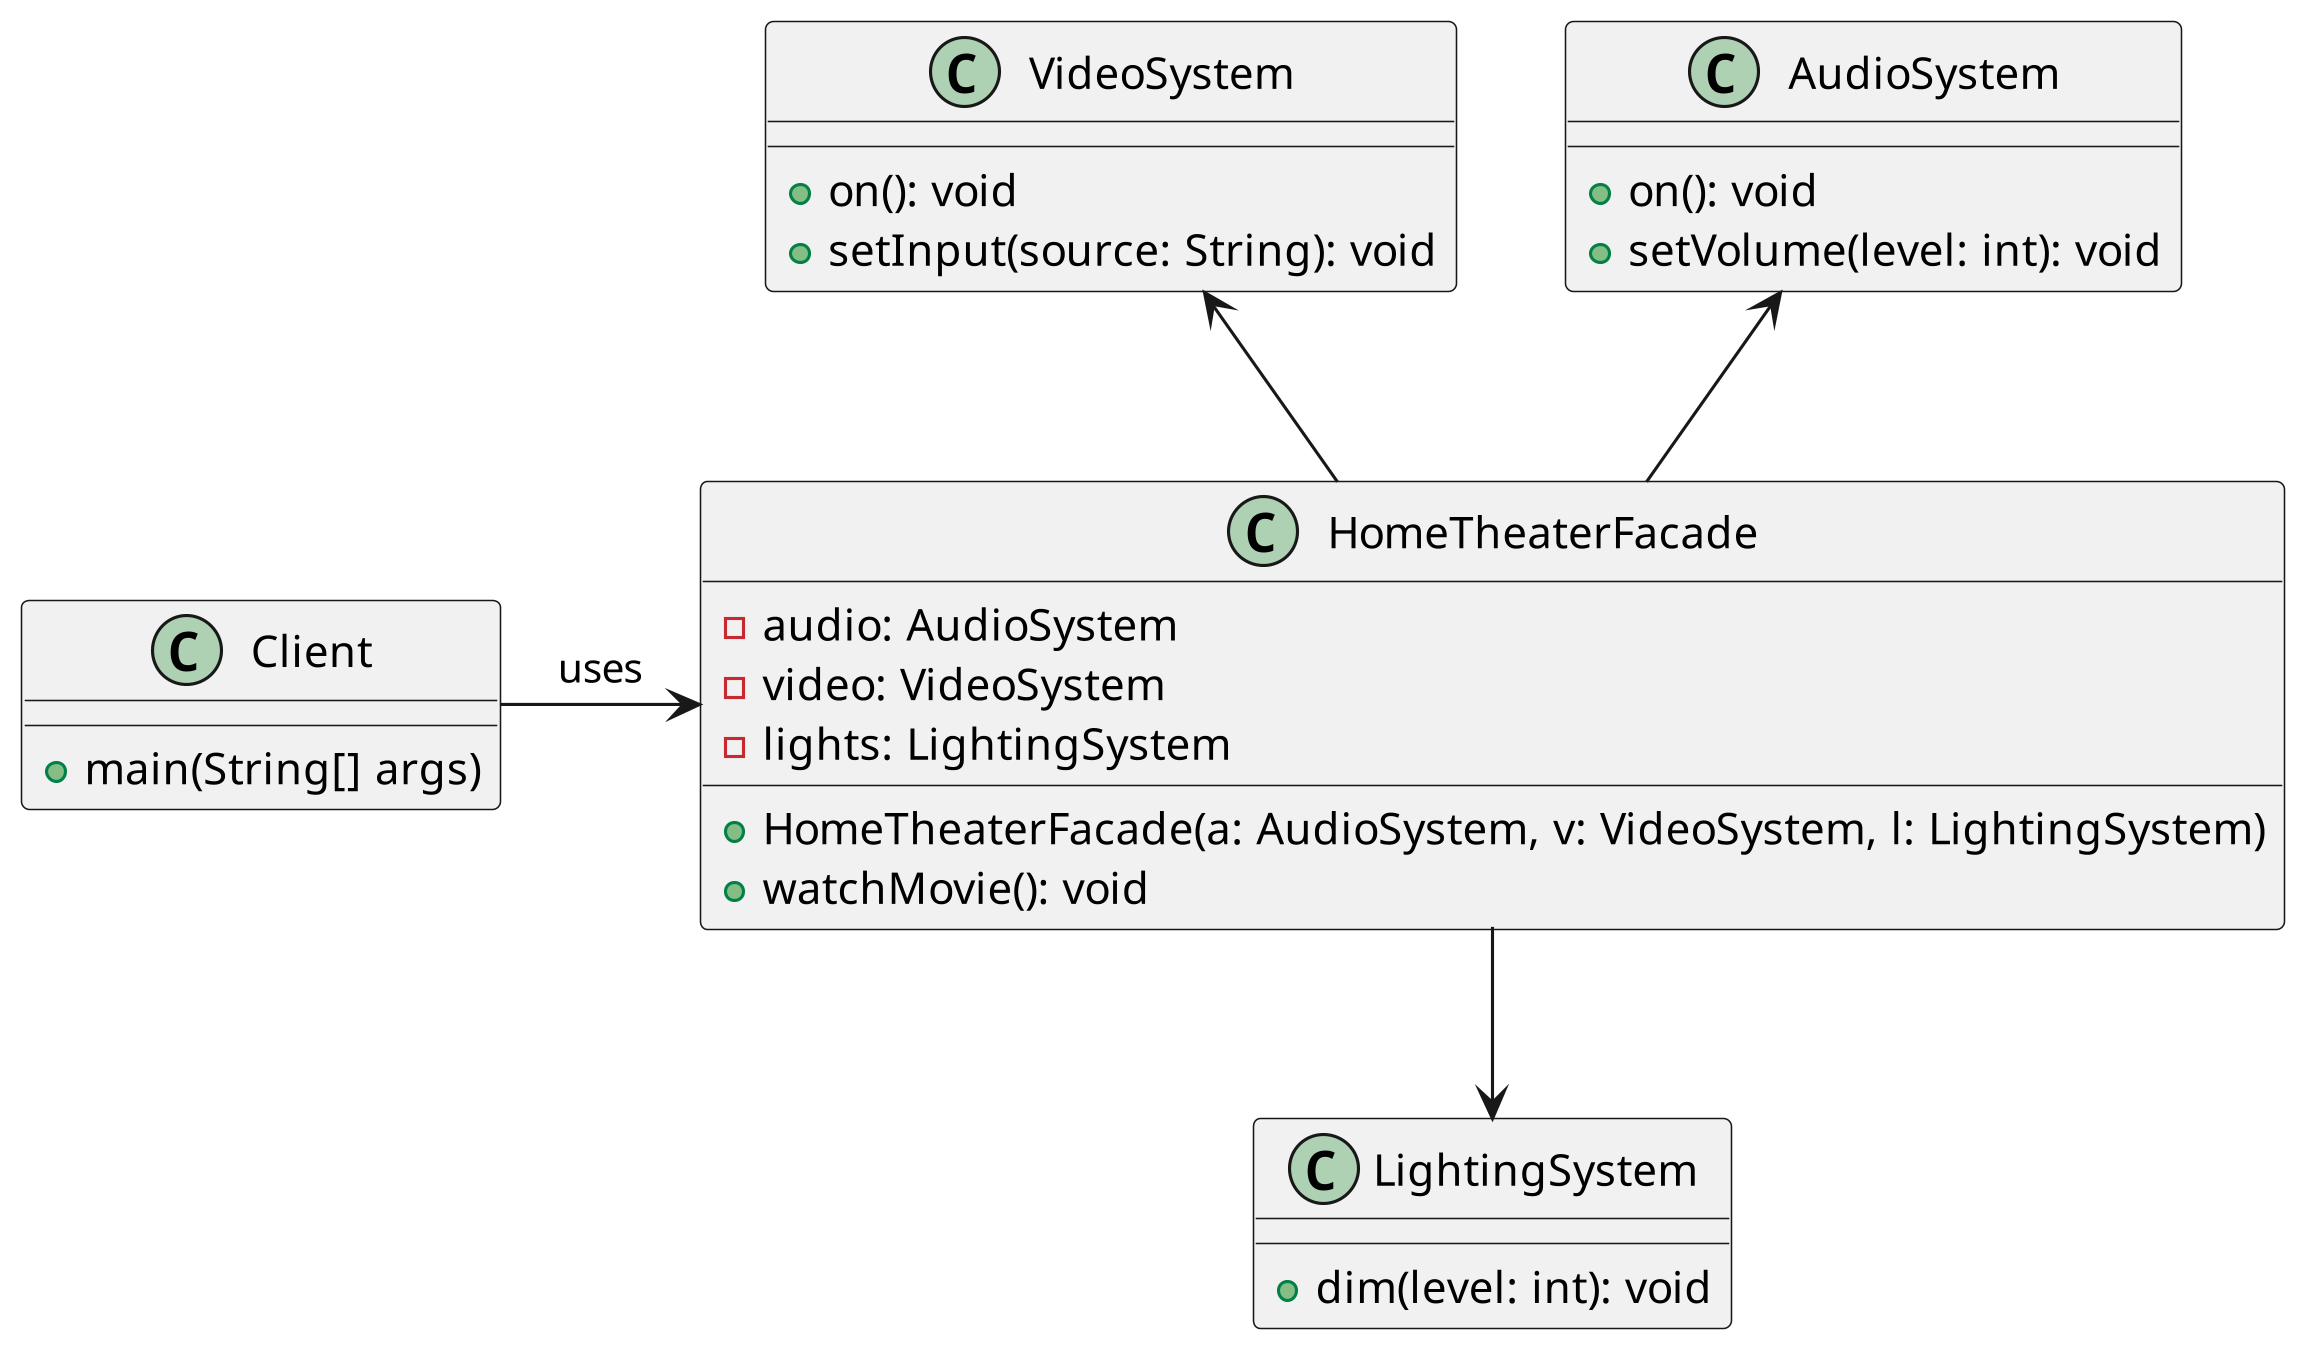
\includegraphics[width=0.7\textwidth]{../../figures/out/facade.png}
	\end{center}
	\small Gambar ini menunjukkan pola \textit{Facade} di mana \texttt{Client} hanya berinteraksi dengan satu objek facade yang menyederhanakan akses ke subsistem.
\end{frame}

\begin{frame}[fragile]{Subsistem: AudioSystem}
\vspace{20pt}
\begin{lstlisting}[style=JavaStyle]
public class AudioSystem {
	public void on() {
		System.out.println("Audio system turned on.");
	}
	public void setVolume(int level) {
		System.out.println("Audio volume set to " + level);
	}
}
\end{lstlisting}
\small Subsistem \texttt{AudioSystem} menyediakan operasi dasar seperti menyalakan dan mengatur volume suara.
\end{frame}

\begin{frame}[fragile]{Subsistem: VideoSystem}
\vspace{20pt}
\begin{lstlisting}[style=JavaStyle]
public class VideoSystem {
	public void on() {
		System.out.println("Video system turned on.");
	}
	public void setInput(String source) {
		System.out.println("Video input set to " + source);
	}
}
\end{lstlisting}
\small \texttt{VideoSystem} menangani konfigurasi sumber input dan aktivasi perangkat video.
\end{frame}

\begin{frame}[fragile]{Subsistem: LightingSystem}
\vspace{20pt}
\begin{lstlisting}[style=JavaStyle]
public class LightingSystem {
	public void dim(int level) {
		System.out.println("Lights dimmed to " + level + "%.");
	}
}
\end{lstlisting}
\small \texttt{LightingSystem} bertugas meredupkan lampu sesuai tingkat kecerahan yang ditentukan.
\end{frame}

\begin{frame}[fragile]{Facade: HomeTheaterFacade}
\begin{columns}[T]
\column{0.5\textwidth}
\begin{lstlisting}[style=JavaStyle, basicstyle=\ttfamily\scriptsize]
public class HomeTheaterFacade {
	private AudioSystem audio;
	private VideoSystem video;
	private LightingSystem lights;
	
	public HomeTheaterFacade(AudioSystem a,
	VideoSystem v,
	LightingSystem l) {
		this.audio = a;
		this.video = v;
		this.lights = l;
	}
\end{lstlisting}

\column{0.5\textwidth}
\begin{lstlisting}[style=JavaStyle, basicstyle=\ttfamily\scriptsize]
	public void watchMovie() {
		lights.dim(30);
		audio.on();
		audio.setVolume(5);
		video.on();
		video.setInput("HDMI1");
		System.out.println(
		"Movie is ready to play.");
	}
}
\end{lstlisting}
\end{columns}

\vspace{5pt}
\small \texttt{HomeTheaterFacade} menyatukan semua subsistem dan menyediakan satu metode \texttt{watchMovie()} untuk klien.
\end{frame}


\begin{frame}[fragile]{Client: Menggunakan Facade}
\vspace{20pt}
\begin{lstlisting}[style=JavaStyle]
public class Main {
	public static void main(String[] args) {
		AudioSystem audio = new AudioSystem();
		VideoSystem video = new VideoSystem();
		LightingSystem lights = new LightingSystem();
		
		HomeTheaterFacade homeTheater = new HomeTheaterFacade(audio, video, lights);
		homeTheater.watchMovie();
	}
}
\end{lstlisting}
\small Klien hanya perlu berinteraksi dengan \texttt{HomeTheaterFacade} tanpa mengetahui cara kerja internal subsistem.
\end{frame}


\section{Pola Proxy}

\begin{frame}{\hfill}
	\centering
	\textbf{\Huge{Pola Proxy}}
\end{frame}

\begin{frame}{Proxy: Tujuan dan Konteks Penggunaan}
	\vspace{20pt}
	\begin{columns}[T,onlytextwidth]
		\column{0.39\textwidth}
		\textbf{Tujuan Utama:}
		\begin{itemize}
			\item Kontrol akses ke objek asli.
			\item Tunda inisialisasi objek berat (lazy).
			\item Tambahkan fungsi tambahan (logging, autentikasi).
		\end{itemize}
		
		\textbf{Kapan Digunakan:}
		\begin{itemize}
			\item Objek mahal atau sensitif.
			\item Perlu kontrol otorisasi pengguna.
			\item Akses objek dari jarak jauh (remote).
		\end{itemize}
		
		\column{0.63\textwidth}
		\textbf{Jenis Proxy:}
		\begin{itemize}
			\item \textbf{Virtual Proxy:} Tunda pembuatan objek besar.
			\item \textbf{Protection Proxy:} Cek hak akses sebelum operasi.
			\item \textbf{Remote Proxy:} Abstraksi objek di server/jaringan.
			\item \textbf{Smart Proxy:} Tambah fitur seperti caching/logging.
		\end{itemize}
		
		\textbf{Contoh Nyata:}
		\begin{itemize}
			\item Lazy loading gambar di UI.
			\item Hibernate proxy untuk entitas database.
			\item Wrapper remote API pada arsitektur microservices.
		\end{itemize}
	\end{columns}
\end{frame}


\begin{frame}{Proxy: Contoh Kasus Penggunaan}
	\vspace{20pt}
	\begin{columns}[T,onlytextwidth]
		\column{0.48\textwidth}
		\textbf{1. Virtual Proxy:} \\
		Tunda pembuatan objek berat seperti \texttt{LargeImage}. Digunakan dalam editor dokumen untuk menghemat memori dan mempercepat loading awal.
		
		\textbf{2. Protection Proxy:} \\
		Batasi akses berdasarkan otorisasi. Misalnya, \texttt{AdminConfigProxy} hanya mengizinkan akses konfigurasi jika pengguna memiliki hak admin.
		
		\textbf{3. Remote Proxy:} \\
		Gunakan proxy untuk mengakses objek di server lain. Digunakan pada RMI, REST API, dan sistem terdistribusi.
		
		\column{0.48\textwidth}
		\textbf{4. Smart Proxy:} \\
		Tambahkan fitur logging, hitung akses, atau validasi tambahan. Cocok untuk aplikasi logistik dan audit.
		
		\textbf{5. Lazy Initialization di ORM:} \\
		Hibernate menggunakan proxy untuk memuat entitas hanya saat dibutuhkan. Ini menghindari pemuatan eager dan meningkatkan performa.
		
		\vspace{10pt}
		\textbf{Kesimpulan:} Proxy membantu mengontrol akses dan menyisipkan logika tambahan tanpa mengubah objek asli atau klien.
	\end{columns}
\end{frame}

\begin{frame}{Proxy: Kelebihan dan Kekurangan}
	\vspace{20pt}
	\begin{columns}[T,onlytextwidth]
		\column{0.5\textwidth}
		\textbf{Kelebihan:}
		\begin{itemize}
			\item \textbf{Kontrol akses terpusat:} Mudah menambahkan otorisasi dan autentikasi.
			\item \textbf{Lazy initialization:} Tunda inisialisasi objek berat sampai diperlukan.
			\item \textbf{Remote access:} Klien tak perlu tahu lokasi fisik objek.
			\item \textbf{Logika tambahan transparan:} Bisa menyisipkan logging, caching, atau audit tanpa ubah objek asli.
			\item \textbf{Pemisahan tanggung jawab:} Objek utama tetap fokus pada logika bisnis.
		\end{itemize}
		
		\column{0.5\textwidth}
		\textbf{Kekurangan:}
		\begin{itemize}
			\item \textbf{Desain lebih kompleks:} Tambahan lapisan bisa memperumit struktur kode.
			\item \textbf{Overhead performa:} Proxy menambah beban pemanggilan metode.
			\item \textbf{Risiko inkonsistensi antarmuka:} Perlu jaga kesesuaian dengan objek asli.
			\item \textbf{Pemeliharaan ganda:} Perlu rawat logika di proxy dan objek asli.
			\item \textbf{Pengujian lebih rumit:} Unit test harus menangani lapisan tambahan.
		\end{itemize}
	\end{columns}
\end{frame}

\begin{frame}{Struktur Pola Proxy}
\vspace{10pt}
\centering
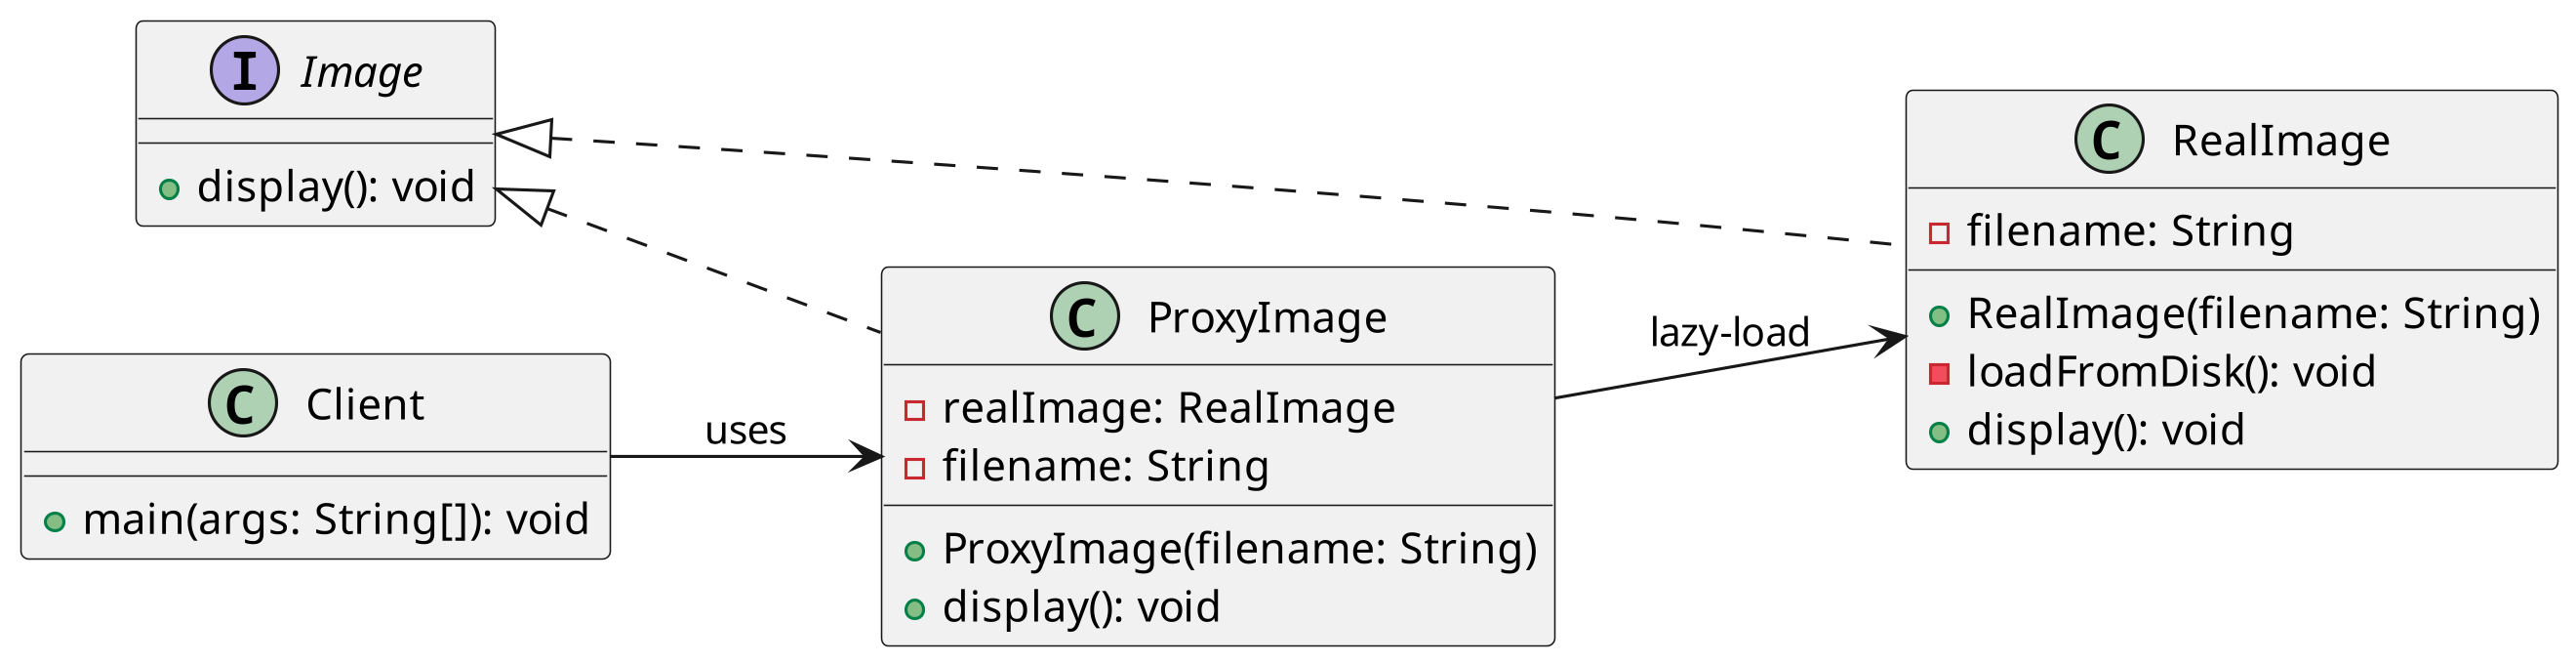
\includegraphics[width=0.9\textwidth]{../../figures/out/proxy.png}
\vspace{10pt}

\small Struktur menunjukkan hubungan antara klien, proxy, dan real subject. Proxy bertindak sebagai perantara antara klien dan objek asli.
\end{frame}

\begin{frame}[fragile]{Proxy - Interface: Image}
\vspace{20pt}
\begin{lstlisting}[style=JavaStyle]
public interface Image {
	void display();
}
\end{lstlisting}

\small Antarmuka \texttt{Image} mendefinisikan kontrak umum yang diimplementasikan oleh \texttt{RealImage} dan \texttt{ProxyImage}.
\end{frame}

\begin{frame}[fragile]{Proxy - RealImage}
\vspace{20pt}
\begin{lstlisting}[style=JavaStyle]
public class RealImage implements Image {
	private String filename;	
	public RealImage(String filename) {
		this.filename = filename;
		loadFromDisk();
	}
	
	private void loadFromDisk() {
		System.out.println("Loading " + filename);
	}
	
	@Override
	public void display() {
		System.out.println("Displaying " + filename);
	}
}
\end{lstlisting}

\small \texttt{RealImage} memuat file saat objek dibuat dan menyediakan metode \texttt{display()} untuk menampilkan gambar.
\end{frame}

\begin{frame}[fragile]{Proxy - ProxyImage}
\vspace{20pt}
\begin{lstlisting}[style=JavaStyle]
public class ProxyImage implements Image {
	private RealImage realImage;
	private String filename;
	
	public ProxyImage(String filename) {
		this.filename = filename;
	}
	
	@Override
	public void display() {
		if (realImage == null) {
			realImage = new RealImage(filename); // Lazy loading
		}
		realImage.display();
	}
}
\end{lstlisting}

\small \texttt{ProxyImage} menunda pembuatan \texttt{RealImage} sampai diperlukan, menghemat sumber daya.
\end{frame}

\begin{frame}[fragile]{Proxy - Client}
\vspace{20pt}
\begin{lstlisting}[style=JavaStyle]
public class Main {
	public static void main(String[] args) {
		Image image = new ProxyImage("photo.jpg");
		
		System.out.println("Proxy created.");
		image.display();
		image.display();
	}
}
\end{lstlisting}

\small Klien menggunakan \texttt{ProxyImage} seperti objek biasa, namun gambar hanya dimuat sekali saat pertama kali digunakan.
\end{frame}

\section{Pola Flyweight}

\begin{frame}{\hfill}
	\centering
	\textbf{\Huge{Pola Flyweight}}
\end{frame}


\begin{frame}{Flyweight: Tujuan dan Konteks Penggunaan}
	\vspace{20pt}
	\begin{columns}[T]
		\column{0.5\textwidth}
		Pola \textit{Flyweight} mengurangi konsumsi memori dan meningkatkan performa dengan membagi objek yang memiliki status internal serupa.
		
		Cocok untuk sistem dengan jutaan objek mirip, seperti teks, grafis, atau partikel dalam game.
		
		\vspace{8pt}
		\textbf{Ciri Flyweight:}
		\begin{itemize}
			\item State bersifat tetap (intrinsik).
			\item State unik dari klien (ekstrinsik).
			\item Objek dibagikan lintas konteks.
		\end{itemize}
		
		\column{0.5\textwidth}
		\textbf{Contoh:}
		\begin{itemize}
			\item Teks: huruf 'a' dipakai berulang.
			\item Game: sprite musuh, peluru dibagikan.
			\item GIS: ikon pohon, gedung, rambu.
			\item Editor: panah, node, label bentuk serupa.
		\end{itemize}
		
		\vspace{5pt}
		\textbf{Manfaat:}
		\begin{itemize}
			\item Hemat memori besar.
			\item Objek instan lebih cepat.
			\item Skala besar lebih efisien.
		\end{itemize}
	\end{columns}
\end{frame}



\begin{frame}{Flyweight: Contoh Kasus Penggunaan}
	\vspace{20pt}
	\begin{columns}[T]
		\column{0.5\textwidth}
		\textbf{1. Rendering Dokumen/Teks}\\
		Editor teks atau browser menggunakan satu objek per karakter untuk menghemat memori. Posisi dan warna disediakan sebagai data eksternal.
		
		\vspace{5pt}
		\textbf{2. Sistem Game}\\
		Peluru, partikel, atau musuh menggunakan flyweight untuk sprite dan animasi. Posisi setiap entitas ditentukan secara terpisah.
		
		\vspace{5pt}
		\textbf{3. Visualisasi Peta (GIS)}\\
		Pohon, gedung, dan rambu jalan menggunakan simbol bersama. Lokasi dan ukuran disimpan di luar objek flyweight.
		
		\column{0.5\textwidth}
		\textbf{4. Editor Grafis}\\
		Panah, node, dan label disimpan sebagai bentuk bersama. Posisi dan rotasi berbeda tiap pemakaian.
		
		\vspace{5pt}
		\textbf{5. Simulasi Agen Massal}\\
		Ribuan agen berbagi model dan animasi dasar. Kecepatan dan tujuan disimpan terpisah.
		
		\vspace{5pt}
		\textbf{6. String Pool di Java}\\
		String literal dengan isi yang sama menunjuk ke objek tunggal dalam pool untuk efisiensi memori dan perbandingan.
	\end{columns}
\end{frame}


\begin{frame}{Flyweight: Kelebihan dan Kekurangan}
	\vspace{20pt}
	\begin{columns}[T]
		\column{0.5\textwidth}
		\textbf{Kelebihan:}
		\begin{itemize}
			\item \textbf{Hemat Memori:} Objek identik dibagikan, menekan penggunaan memori.
			\item \textbf{Kinerja Meningkat:} Alokasi objek dan GC lebih ringan.
			\item \textbf{Pemisahan State:} Mendorong desain antara data statis dan dinamis.
			\item \textbf{Skalabilitas Tinggi:} Mendukung jutaan objek tanpa membebani sistem.
			\item \textbf{Didukung Sistem:} Java String Pool dan Glyph Cache adalah contoh umum.
		\end{itemize}
		
		\column{0.5\textwidth}
		\textbf{Kekurangan:}
		\begin{itemize}
			\item \textbf{State Eksternal Harus Konsisten:} Pengembang harus hati-hati.
			\item \textbf{Kode Lebih Rumit:} Pemisahan state menambah beban desain.
			\item \textbf{Tidak Efektif untuk Objek Unik:} Flyweight kurang bermanfaat bila objek terlalu bervariasi.
			\item \textbf{Perlu Sinkronisasi:} Untuk multithreading, thread-safety harus dijaga.
			\item \textbf{Debugging Lebih Sulit:} Objek bersama menyulitkan pelacakan perilaku.
		\end{itemize}
	\end{columns}
\end{frame}


\begin{frame}[fragile]{Flyweight: Struktur Implementasi (Diagram)}
	\vspace{10pt}
	\centering
	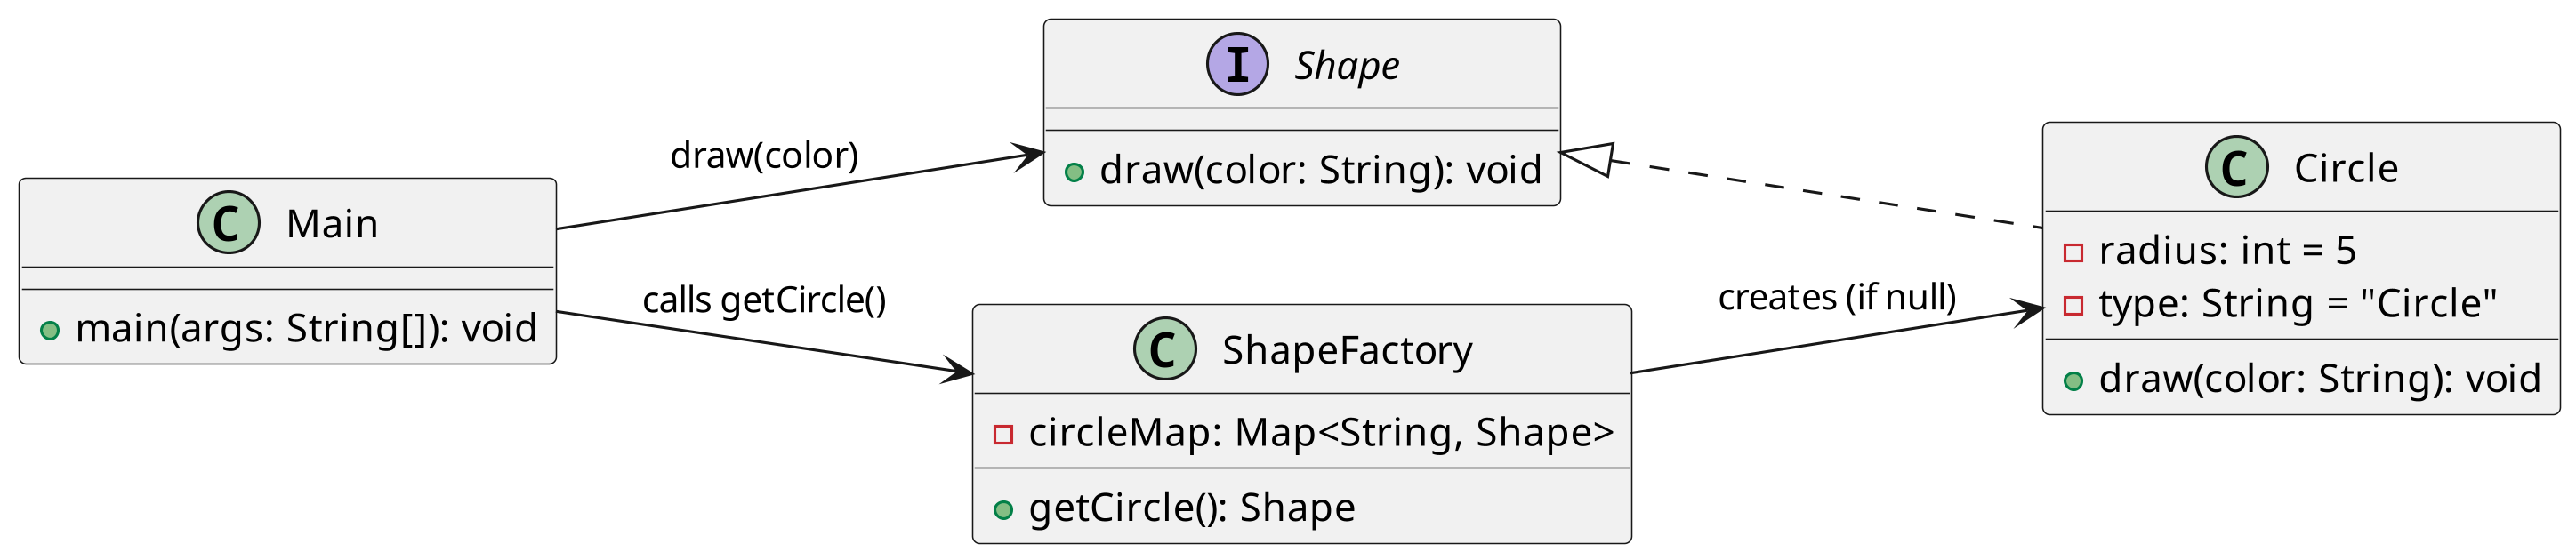
\includegraphics[width=0.9\textwidth]{../../figures/out/flyweight.png}
	\vspace{10pt}
	
	\small Gambar menunjukkan hubungan antara klien, flyweight, dan \texttt{ShapeFactory} yang mengelola objek bersama (\textit{shared}).
\end{frame}

\begin{frame}[fragile]{Flyweight: Interface \texttt{Shape}}
\vspace{10pt}
\begin{lstlisting}[style=JavaStyle]
public interface Shape {
	void draw(String color); // color = ekstrinsik
}
\end{lstlisting}
\small \texttt{Shape} mendefinisikan antarmuka umum untuk semua objek flyweight dan menerima state eksternal sebagai parameter.
\end{frame}

\begin{frame}[fragile]{Flyweight: Implementasi \texttt{Circle}}
\vspace{10pt}
\begin{lstlisting}[style=JavaStyle]
public class Circle implements Shape {
	private final int radius = 5; // intrinsik
	private final String type = "Circle"; // intrinsik
	
	@Override
	public void draw(String color) {
		System.out.println("Drawing " + type + 
		" with radius " + radius + " and color " + color);
	}
}
\end{lstlisting}
\small \texttt{Circle} menyimpan informasi yang tidak berubah, sementara warna diberikan saat digunakan.
\end{frame}

\begin{frame}[fragile]{Flyweight: \texttt{ShapeFactory}}
\vspace{10pt}
\begin{lstlisting}[style=JavaStyle]
import java.util.HashMap;
import java.util.Map;

public class ShapeFactory {
	private static final Map<String, Shape> circleMap = new HashMap<>();
	
	public static Shape getCircle() {
		Shape circle = circleMap.get("circle");
		if (circle == null) {
			circle = new Circle();
			circleMap.put("circle", circle);
			System.out.println("Creating new Circle instance.");
		}
		return circle;
	}
}
\end{lstlisting}
\small \texttt{ShapeFactory} berperan sebagai cache: hanya membuat satu instance dan mendistribusikan ulang jika dibutuhkan.
\end{frame}

\begin{frame}[fragile]{Flyweight: Client}
\vspace{10pt}
\begin{lstlisting}[style=JavaStyle]
public class Main {
	public static void main(String[] args) {
		String[] colors = { "Red", "Green", "Blue", "Yellow" };
		
		for (int i = 0; i < 10; i++) {
			Shape circle = ShapeFactory.getCircle();
			circle.draw(colors[i % colors.length]); // ekstrinsik
		}
	}
}
\end{lstlisting}
\small Meskipun hanya satu objek \texttt{Circle} dibuat, ia digunakan untuk menggambar 10 kali dengan warna berbeda.
\end{frame}

\begin{frame}{Kesimpulan}
	\vspace{10pt}
	\begin{columns}[T]
		\column{0.5\textwidth}
		\textbf{Pola dan Tujuan:}
		\begin{itemize}
			\item \textbf{Facade:} Satu antarmuka ke subsistem kompleks.
			\item \textbf{Proxy:} Kendali/perwakilan objek lain.
			\item \textbf{Flyweight:} Berbagi objek identik hemat memori.
		\end{itemize}
		
		\vspace{4pt}
		\textbf{Manfaat Umum:}
		\begin{itemize}
			\item Modularitas dan keterpisahan meningkat.
			\item Pemeliharaan dan pengujian lebih mudah.
			\item Cocok untuk sistem scalable.
		\end{itemize}
		
		\column{0.5\textwidth}
		\textbf{Aplikasi dan Catatan:}
		\begin{itemize}
			\item \textit{Facade} untuk simplifikasi layanan.
			\item \textit{Proxy} untuk proteksi dan akses tak langsung.
			\item \textit{Flyweight} pada grafis, teks, objek berulang.
			\item Pilih pola sesuai kebutuhan dan kompleksitas.
		\end{itemize}
		
		\vspace{4pt}
		\textbf{Penutup:}
		\begin{itemize}
			\item Pola ini memperkuat desain berorientasi objek.
			\item Gunakan untuk sistem fleksibel dan efisien.
		\end{itemize}
	\end{columns}
\end{frame}





\end{document}
                                                                                                                                                                               